% Edit only the text between matching begin and end lines.
\documentclass[11pt,a4paper]{article}
% Shared preamble for TMUA question papers. Local edits here are overwritten.

% Reproducible PDFs: no timestamps, no trailer id, no build-path details.
\ifdefined\pdfsuppressptexinfo
  \pdfsuppressptexinfo=-1
  \pdfinfoomitdate=1
  \pdftrailerid{}
\fi

\usepackage{graphicx}
\usepackage{mathtools}
\usepackage{amssymb}
\usepackage{amsmath}
\usepackage{amsthm}
\usepackage{enumitem}
\usepackage{microtype}
\usepackage[table]{xcolor}
\usepackage{array}
\usepackage{booktabs}
\usepackage{tabularx}
\usepackage{longtable}
\usepackage{ragged2e}
\usepackage{fancyhdr}
\usepackage{etoolbox}
\usepackage[
  a4paper,
  left=0.8in,
  right=1in,
  top=1in,
  bottom=0.5in,
  headheight=14pt,
  headsep=0.4in
]{geometry}

\usepackage{pgfplots}
\pgfplotsset{compat=1.18}
\usepgfplotslibrary{fillbetween, polar}
\usetikzlibrary{calc, positioning}
\usetikzlibrary{angles, quotes}
\usetikzlibrary{arrows.meta}
\usetikzlibrary{decorations.pathreplacing, decorations.markings}
\usetikzlibrary{patterns}
\usetikzlibrary{intersections}

\usepackage{tocloft}
\usepackage[hidelinks]{hyperref}
\hypersetup{pdfauthor={danieljsmith.org}, pdfcreator={}, pdfsubject={}, pdfkeywords={}}
\urlstyle{same}
\tocloftpagestyle{djspaper}
\setlength{\cftbeforesubsecskip}{2pt}
\setlength{\cftsubsecindent}{1.5em}
\setlength{\cftsubsecnumwidth}{0pt}
\renewcommand{\cftsubsecfont}{\small\color{black}}
\renewcommand{\cftsubsecpagefont}{\small\color{black}}
\renewcommand{\cftsubsecleader}{\hfill}

% \djsPaperSetup{<PDF title>}{<header label>}, called once after this file.
\newcommand{\djsHeaderLabel}{}
\newcommand{\djsPaperSetup}[2]{%
  \hypersetup{pdftitle={#1}}%
  \renewcommand{\djsHeaderLabel}{#2}}

\setlength{\parindent}{0pt}
\fancypagestyle{djspaper}{%
  \fancyhead{}%
  \fancyfoot{}%
  \renewcommand{\headrulewidth}{0.9pt}%
  \fancyhead[L]{\djsHeaderLabel}%
  \fancyhead[R]{\href{https://danieljsmith.org}{danieljsmith.org}}%
}
\pagestyle{djspaper}

\newcolumntype{Y}{>{\RaggedRight\arraybackslash}X}

% Topic labels: a subtle line above each question and a suffix on its
% contents entry. The bookmark form is spelled out separately, because a PDF
% bookmark is plain text and would otherwise keep the colour name.
\newcommand{\djsTocTopic}[1]{%
  \ifblank{#1}{}{%
    \texorpdfstring
      {\hspace{0.9em}{\footnotesize\itshape\color{black!45}#1}}
      { \textendash\ #1}}}
\newcommand{\djsTopicLine}[1]{%
  \ifblank{#1}{}{%
    {\raggedleft\footnotesize\itshape\color{black!45}#1\par}%
    \vspace{-0.6\baselineskip}}}

\newcommand{\questionitem}[1][]{%
  \item\phantomsection
  \addcontentsline{toc}{subsection}{%
    Question \number\value{enumi}\protect\djsTocTopic{#1}}%
}
\renewcommand{\contentsname}{Questions}
\newcommand{\djsFrontMatter}{%
  \vspace*{20pt}%
  \tableofcontents
  \newpage
}

\djsPaperSetup{TMUA Set A Paper 1}{TMUA Set A - Paper 1}
\begin{document}
\thispagestyle{djspaper}
\djsFrontMatter
\thispagestyle{djspaper}
\vspace*{8pt}
\djsTopicLine{Exponentials \& Logarithms}
\begin{enumerate}[label=\textbf{\arabic*.},leftmargin=*,itemsep=0pt,start=1]
\questionitem[Exponentials \& Logarithms]
% begin q000607 stem
Find the complete set of positive real values of $x$, with $x \neq 1$, for which\[\log_2 x < \log_x 2\]
% end q000607 stem

\par\vspace*{12pt}
\begin{tabularx}{\linewidth}{@{}>{\bfseries}l Y@{}}
A &
% begin q000607 choice A
$0<x<\frac{1}{2}$ or $1<x<2$
% end q000607 choice A
\\[0.8em]
B &
% begin q000607 choice B
$\frac{1}{2}<x<1$ or $x>2$
% end q000607 choice B
\\[0.8em]
C &
% begin q000607 choice C
$1<x<2$
% end q000607 choice C
\\[0.8em]
D &
% begin q000607 choice D
$0<x<\frac{1}{2}$
% end q000607 choice D
\\[0.8em]
E &
% begin q000607 choice E
$0<x<1$ or $x>2$
% end q000607 choice E
\\[0.8em]
F &
% begin q000607 choice F
$x>2$
% end q000607 choice F
\\[0.8em]
G &
% begin q000607 choice G
$0<x<2$, $x \neq 1$
% end q000607 choice G
\\
\end{tabularx}
\end{enumerate}
\clearpage
\thispagestyle{djspaper}
\vspace*{8pt}
\djsTopicLine{Inequalities}
\begin{enumerate}[label=\textbf{\arabic*.},leftmargin=*,itemsep=0pt,start=2]
\questionitem[Inequalities]
% begin q000029 stem
Fix a real number $a\ne 0$.

Consider the inequality \[ |x-a|+|x+a|<3|a| \] Which of the following describes the set of all real $x$ satisfying the inequality?
% end q000029 stem

\par\vspace*{12pt}
\begin{tabularx}{\linewidth}{@{}>{\bfseries}l Y@{}}
A &
% begin q000029 choice A
No real solutions
% end q000029 choice A
\\[0.8em]
B &
% begin q000029 choice B
All real $x$ with $|x|<|a|$
% end q000029 choice B
\\[0.8em]
C &
% begin q000029 choice C
All real $x$ with $|x|<\dfrac{3|a|}{2}$
% end q000029 choice C
\\[0.8em]
D &
% begin q000029 choice D
All real $x$ with $|x|<3|a|$
% end q000029 choice D
\\[0.8em]
E &
% begin q000029 choice E
All real $x$ with $\dfrac{|a|}{2}<|x|<\dfrac{3|a|}{2}$
% end q000029 choice E
\\
\end{tabularx}
\end{enumerate}
\clearpage
\thispagestyle{djspaper}
\vspace*{8pt}
\djsTopicLine{Differentiation}
\begin{enumerate}[label=\textbf{\arabic*.},leftmargin=*,itemsep=0pt,start=3]
\questionitem[Differentiation]
% begin q000624 stem
The diagram shows parts of the curves $y=x^2$ and $y=(x-2)^2+b$, where $b$ is positive. 

The curves meet at $P$, and the tangents to the curves at $P$ are perpendicular.

What is the value of $b$?
% end q000624 stem

\begin{center}
% begin q000624 diagram
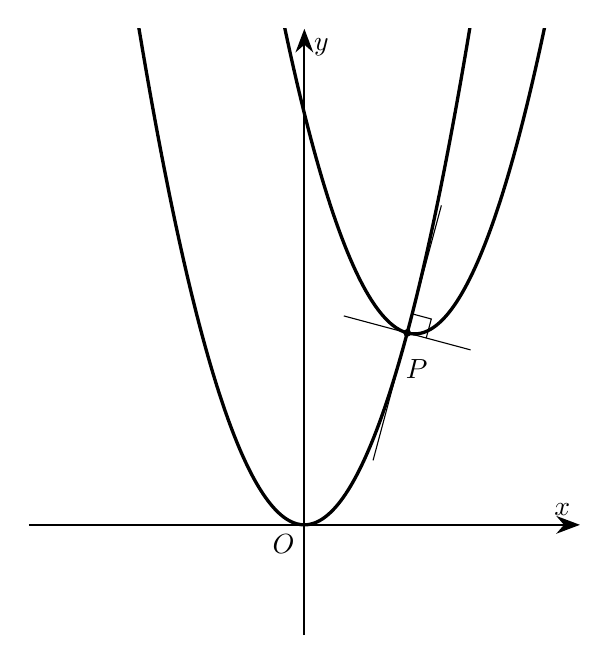
\begin{tikzpicture}
\pgfmathsetmacro{\px}{1+sqrt(3)/2}
\pgfmathsetmacro{\py}{\px*\px}
\pgfmathsetmacro{\bshift}{4*(\px-1)}
\pgfmathsetmacro{\mone}{2*\px}
\pgfmathsetmacro{\mtwo}{2*(\px-2)}
\pgfmathsetmacro{\tone}{0.62}
\pgfmathsetmacro{\ttwo}{1.15}
\pgfmathsetmacro{\tOnePX}{\px+\tone}
\pgfmathsetmacro{\tOnePY}{\py+\tone*\mone}
\pgfmathsetmacro{\tOneMX}{\px-\tone}
\pgfmathsetmacro{\tOneMY}{\py-\tone*\mone}
\pgfmathsetmacro{\tTwoPX}{\px+\ttwo}
\pgfmathsetmacro{\tTwoPY}{\py+\ttwo*\mtwo}
\pgfmathsetmacro{\tTwoMX}{\px-\ttwo}
\pgfmathsetmacro{\tTwoMY}{\py-\ttwo*\mtwo}
\begin{axis}[
    axis lines=middle,
    axis line style={thick,-{Stealth[length=3mm]}},
    xlabel={$x$},
    ylabel={$y$},
    xmin=-5, xmax=5,
    ymin=-2, ymax=9,
    xtick=\empty,
    ytick=\empty,
    width=7cm,
    height=12cm,
    scale only axis,
    axis equal image,
    enlargelimits=false,
    clip=true,
    samples=180
]
\addplot[very thick, black, domain=-4:3.2]
    {x^2}
    node[pos=0.12, above right] {$y=x^2$};
\addplot[very thick, black, domain=-1.2:5]
    {(x-2)^2+\bshift}
    node[pos=0.145, above right] {$y=(x-2)^2+b$};

\coordinate (P) at (axis cs:\px,\py);
\coordinate (TOnePlus) at (axis cs:\tOnePX,\tOnePY);
\coordinate (TOneMinus) at (axis cs:\tOneMX,\tOneMY);
\coordinate (TTwoPlus) at (axis cs:\tTwoPX,\tTwoPY);
\coordinate (TTwoMinus) at (axis cs:\tTwoMX,\tTwoMY);

\draw[thin, black] (TOneMinus) -- (TOnePlus);
\draw[thin, black] (TTwoMinus) -- (TTwoPlus);
\pic[draw, thin, angle radius=2.5mm]
    {right angle=TTwoPlus--P--TOnePlus};

\fill[black] (P) circle (1.4pt);
\node[anchor=south west, xshift=-4pt, yshift=-20pt] at (P) {$P$};
\node[below left] at (axis cs:0,0) {$O$};
\end{axis}
\end{tikzpicture}
% end q000624 diagram
\end{center}

\par\vspace*{12pt}
\begin{tabularx}{\linewidth}{@{}>{\bfseries}l Y@{}}
A &
% begin q000624 choice A
$\dfrac{\sqrt{3}}{2}$
% end q000624 choice A
\\[0.8em]
B &
% begin q000624 choice B
$\sqrt{3}$
% end q000624 choice B
\\[0.8em]
C &
% begin q000624 choice C
$2\sqrt{3}$
% end q000624 choice C
\\[0.8em]
D &
% begin q000624 choice D
$3\sqrt{3}$
% end q000624 choice D
\\[0.8em]
E &
% begin q000624 choice E
$4\sqrt{3}$
% end q000624 choice E
\\
\end{tabularx}
\end{enumerate}
\clearpage
\thispagestyle{djspaper}
\vspace*{8pt}
\djsTopicLine{Algebra}
\begin{enumerate}[label=\textbf{\arabic*.},leftmargin=*,itemsep=0pt,start=4]
\questionitem[Algebra]
% begin q000586 stem
A positive real number $x$ satisfies
\[
(x-2)(x+3)(x+4)(x+9)=3024
\]
What is the value of $x^2+7x$?
% end q000586 stem

\par\vspace*{12pt}
\begin{tabularx}{\linewidth}{@{}>{\bfseries}l Y@{}}
A &
% begin q000586 choice A
$16$
% end q000586 choice A
\\[0.8em]
B &
% begin q000586 choice B
$38$
% end q000586 choice B
\\[0.8em]
C &
% begin q000586 choice C
$54$
% end q000586 choice C
\\[0.8em]
D &
% begin q000586 choice D
$60$
% end q000586 choice D
\\[0.8em]
E &
% begin q000586 choice E
$114$
% end q000586 choice E
\\
\end{tabularx}
\end{enumerate}
\clearpage
\thispagestyle{djspaper}
\vspace*{8pt}
\djsTopicLine{Integration}
\begin{enumerate}[label=\textbf{\arabic*.},leftmargin=*,itemsep=0pt,start=5]
\questionitem[Integration]
% begin q000603 stem
The curve $y = x^3 - 3x + 5$ has a tangent line at the point where $x = 2$. 

This tangent meets the curve again at exactly one other point. Find the area of the region enclosed between the curve and the tangent.
% end q000603 stem

\par\vspace*{12pt}
\begin{tabularx}{\linewidth}{@{}>{\bfseries}l Y@{}}
A &
% begin q000603 choice A
$-108$
% end q000603 choice A
\\[0.8em]
B &
% begin q000603 choice B
$54$
% end q000603 choice B
\\[0.8em]
C &
% begin q000603 choice C
$96$
% end q000603 choice C
\\[0.8em]
D &
% begin q000603 choice D
$108$
% end q000603 choice D
\\[0.8em]
E &
% begin q000603 choice E
$120$
% end q000603 choice E
\\[0.8em]
F &
% begin q000603 choice F
$216$
% end q000603 choice F
\\
\end{tabularx}
\end{enumerate}
\clearpage
\thispagestyle{djspaper}
\vspace*{8pt}
\djsTopicLine{Coordinate Geometry}
\begin{enumerate}[label=\textbf{\arabic*.},leftmargin=*,itemsep=0pt,start=6]
\questionitem[Coordinate Geometry]
% begin q000633 stem
A straight line passes through the point $(2, 5)$ and has gradient $m$.

The line forms a triangle of area $25$ with the positive $x$-axis and the positive $y$-axis.

What is the sum of all possible values of $m$?
% end q000633 stem

\par\vspace*{12pt}
\begin{tabularx}{\linewidth}{@{}>{\bfseries}l Y@{}}
A &
% begin q000633 choice A
$-15$
% end q000633 choice A
\\[0.8em]
B &
% begin q000633 choice B
$-\dfrac{15}{2}$
% end q000633 choice B
\\[0.8em]
C &
% begin q000633 choice C
$-\dfrac{25}{4}$
% end q000633 choice C
\\[0.8em]
D &
% begin q000633 choice D
$-\dfrac{15}{4}$
% end q000633 choice D
\\[0.8em]
E &
% begin q000633 choice E
$\dfrac{15}{2}$
% end q000633 choice E
\\
\end{tabularx}
\end{enumerate}
\clearpage
\thispagestyle{djspaper}
\vspace*{8pt}
\djsTopicLine{Number}
\begin{enumerate}[label=\textbf{\arabic*.},leftmargin=*,itemsep=0pt,start=7]
\questionitem[Number]
% begin q000641 stem
Consider the integer
\[N = 8^{15}\times 5^{40}\]
When $N$ is written out in full, how many digits does it have?
% end q000641 stem

\par\vspace*{12pt}
\begin{tabularx}{\linewidth}{@{}>{\bfseries}l Y@{}}
A &
% begin q000641 choice A
$40$
% end q000641 choice A
\\[0.8em]
B &
% begin q000641 choice B
$41$
% end q000641 choice B
\\[0.8em]
C &
% begin q000641 choice C
$42$
% end q000641 choice C
\\[0.8em]
D &
% begin q000641 choice D
$43$
% end q000641 choice D
\\[0.8em]
E &
% begin q000641 choice E
$46$
% end q000641 choice E
\\[0.8em]
F &
% begin q000641 choice F
$55$
% end q000641 choice F
\\
\end{tabularx}
\end{enumerate}
\clearpage
\thispagestyle{djspaper}
\vspace*{8pt}
\djsTopicLine{Sequences \& Series}
\begin{enumerate}[label=\textbf{\arabic*.},leftmargin=*,itemsep=0pt,start=8]
\questionitem[Sequences \& Series]
% begin q000650 stem
The $n$th term of a sequence is a quadratic expression in $n$. 

The second, fifth and eighth terms are $4$, $13$ and $40$, respectively. 

What is the eleventh term?
% end q000650 stem

\par\vspace*{12pt}
\begin{tabularx}{\linewidth}{@{}>{\bfseries}l Y@{}}
A &
% begin q000650 choice A
$67$
% end q000650 choice A
\\[0.8em]
B &
% begin q000650 choice B
$76$
% end q000650 choice B
\\[0.8em]
C &
% begin q000650 choice C
$85$
% end q000650 choice C
\\[0.8em]
D &
% begin q000650 choice D
$94$
% end q000650 choice D
\\[0.8em]
E &
% begin q000650 choice E
$121$
% end q000650 choice E
\\
\end{tabularx}
\end{enumerate}
\clearpage
\thispagestyle{djspaper}
\vspace*{8pt}
\djsTopicLine{Geometry}
\begin{enumerate}[label=\textbf{\arabic*.},leftmargin=*,itemsep=0pt,start=9]
\questionitem[Geometry]
% begin q000635 stem
A circle of radius $1$ lies in the region where $x\ge 0$ and $y\ge 0$, and touches both axes.

A second, smaller circle also lies in this region, touches both axes, and touches the first circle at exactly one point. 

The two circles do not overlap.

What is the radius of the smaller circle?
% end q000635 stem

\begin{center}
% begin q000635 diagram
\begin{tikzpicture}[scale=2.5]
\def\R{1}
\def\xmax{2.6}
\def\ymax{2.6}
\pgfmathsetmacro{\rsmall}{\R*(sqrt(2)-1)/(sqrt(2)+1)}

\coordinate (O) at (0,0);
\coordinate (C) at (\R,\R);
\coordinate (D) at (\rsmall,\rsmall);
\coordinate (B) at (\R,0);
\coordinate (T) at ($(D)+(45:\rsmall)$);

\draw[-{Stealth[length=3mm]}] (O) -- (\xmax,0) node[right] {$x$};
\draw[-{Stealth[length=3mm]}] (O) -- (0,\ymax) node[above] {$y$};

\draw[thick, black] (C) circle (\R);
\draw[thick, black] (D) circle (\rsmall);

\end{tikzpicture}
% end q000635 diagram
\end{center}

\par\vspace*{12pt}
\begin{tabularx}{\linewidth}{@{}>{\bfseries}l Y@{}}
A &
% begin q000635 choice A
$\dfrac{1}{3}$
% end q000635 choice A
\\[0.8em]
B &
% begin q000635 choice B
$3-2\sqrt{2}$
% end q000635 choice B
\\[0.8em]
C &
% begin q000635 choice C
$\sqrt{2}-1$
% end q000635 choice C
\\[0.8em]
D &
% begin q000635 choice D
$\dfrac{\sqrt{2}-1}{2}$
% end q000635 choice D
\\[0.8em]
E &
% begin q000635 choice E
$2-\sqrt{2}$
% end q000635 choice E
\\[0.8em]
F &
% begin q000635 choice F
$17-12\sqrt{2}$
% end q000635 choice F
\\[0.8em]
G &
% begin q000635 choice G
$3+2\sqrt{2}$
% end q000635 choice G
\\
\end{tabularx}
\end{enumerate}
\clearpage
\thispagestyle{djspaper}
\vspace*{8pt}
\djsTopicLine{Sequences \& Series}
\begin{enumerate}[label=\textbf{\arabic*.},leftmargin=*,itemsep=0pt,start=10]
\questionitem[Sequences \& Series]
% begin q000048 stem
A sequence $a_n$ is defined by $a_0=3$ and, for $n\ge 0$, \[ a_{n+1}=3(a_n)^2 \] Which of the following is equal to $\log_3(a_n)$?
% end q000048 stem

\par\vspace*{12pt}
\begin{tabularx}{\linewidth}{@{}>{\bfseries}l Y@{}}
A &
% begin q000048 choice A
$2^n$
% end q000048 choice A
\\[0.8em]
B &
% begin q000048 choice B
$2^n-1$
% end q000048 choice B
\\[0.8em]
C &
% begin q000048 choice C
$2^{n+1}-1$
% end q000048 choice C
\\[0.8em]
D &
% begin q000048 choice D
$2^{n+1}+1$
% end q000048 choice D
\\[0.8em]
E &
% begin q000048 choice E
$2^{n}-2$
% end q000048 choice E
\\[0.8em]
F &
% begin q000048 choice F
$2^{n+1}-2$
% end q000048 choice F
\\
\end{tabularx}
\end{enumerate}
\clearpage
\thispagestyle{djspaper}
\vspace*{8pt}
\djsTopicLine{Number}
\begin{enumerate}[label=\textbf{\arabic*.},leftmargin=*,itemsep=0pt,start=11]
\questionitem[Number]
% begin q000567 stem
An integer $n$ is chosen at random from the integers $1$ to $1260$ inclusive, with each integer equally likely to be chosen. 

The fraction $\dfrac{n}{1260}$ is written as a decimal.

What is the probability that this decimal terminates and that its shortest form has exactly two digits after the decimal point?

In the shortest form, zeros at the end are omitted; for example, $0.50$ is written as $0.5$.
% end q000567 stem

\par\vspace*{12pt}
\begin{tabularx}{\linewidth}{@{}>{\bfseries}l Y@{}}
A &
% begin q000567 choice A
$\dfrac{1}{630}$
% end q000567 choice A
\\[0.8em]
B &
% begin q000567 choice B
$\dfrac{2}{315}$
% end q000567 choice B
\\[0.8em]
C &
% begin q000567 choice C
$\dfrac{1}{126}$
% end q000567 choice C
\\[0.8em]
D &
% begin q000567 choice D
$\dfrac{1}{90}$
% end q000567 choice D
\\[0.8em]
E &
% begin q000567 choice E
$\dfrac{1}{70}$
% end q000567 choice E
\\[0.8em]
F &
% begin q000567 choice F
$\dfrac{1}{63}$
% end q000567 choice F
\\
\end{tabularx}
\end{enumerate}
\clearpage
\thispagestyle{djspaper}
\vspace*{8pt}
\djsTopicLine{Functions \& Graphs}
\begin{enumerate}[label=\textbf{\arabic*.},leftmargin=*,itemsep=0pt,start=12]
\questionitem[Functions \& Graphs]
% begin q000573 stem
A function $f$ has the form $f(x)=ax+b$, where $a$ and $b$ are real constants.

For every real $x$, applying $f$ twice gives
\[
f(f(x))=4x+3
\]

What is the difference between the greatest and least possible values of $f(2)$?
% end q000573 stem

\par\vspace*{12pt}
\begin{tabularx}{\linewidth}{@{}>{\bfseries}l Y@{}}
A &
% begin q000573 choice A
$2$
% end q000573 choice A
\\[0.8em]
B &
% begin q000573 choice B
$4$
% end q000573 choice B
\\[0.8em]
C &
% begin q000573 choice C
$7$
% end q000573 choice C
\\[0.8em]
D &
% begin q000573 choice D
$10$
% end q000573 choice D
\\[0.8em]
E &
% begin q000573 choice E
$12$
% end q000573 choice E
\\[0.8em]
F &
% begin q000573 choice F
$14$
% end q000573 choice F
\\
\end{tabularx}
\end{enumerate}
\clearpage
\thispagestyle{djspaper}
\vspace*{8pt}
\djsTopicLine{Algebra}
\begin{enumerate}[label=\textbf{\arabic*.},leftmargin=*,itemsep=0pt,start=13]
\questionitem[Algebra]
% begin q000595 stem
The equation $x^2-7x+1=0$ has two positive solutions, $p$ and $q$.

What is the value of

\[ \frac{p-1}{p+1}\times\frac{q-1}{q+1} \,\, \mathrm{?}\]
% end q000595 stem

\par\vspace*{12pt}
\begin{tabularx}{\linewidth}{@{}>{\bfseries}l Y@{}}
A &
% begin q000595 choice A
$-\dfrac{2}{3}$
% end q000595 choice A
\\[0.8em]
B &
% begin q000595 choice B
$-\dfrac{5}{8}$
% end q000595 choice B
\\[0.8em]
C &
% begin q000595 choice C
$-\dfrac{5}{9}$
% end q000595 choice C
\\[0.8em]
D &
% begin q000595 choice D
$\dfrac{5}{9}$
% end q000595 choice D
\\[0.8em]
E &
% begin q000595 choice E
$\dfrac{5}{8}$
% end q000595 choice E
\\[0.8em]
F &
% begin q000595 choice F
$\dfrac{2}{3}$
% end q000595 choice F
\\
\end{tabularx}
\end{enumerate}
\clearpage
\thispagestyle{djspaper}
\vspace*{8pt}
\djsTopicLine{Probability \& Counting}
\begin{enumerate}[label=\textbf{\arabic*.},leftmargin=*,itemsep=0pt,start=14]
\questionitem[Probability \& Counting]
% begin q000658 stem
A cube has edge length $1$. 

Three different vertices are chosen at random. 

Every choice of three vertices is equally likely.

What is the probability that the three chosen vertices form a right-angled triangle?
% end q000658 stem

\begin{center}
% begin q000658 diagram
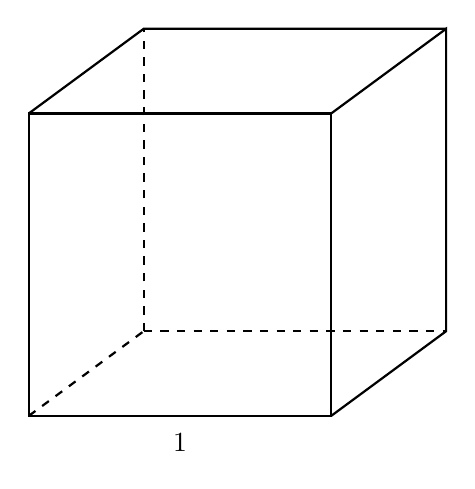
\begin{tikzpicture}[
    scale=1.2,
    x={(1cm,0cm)},
    y={(0.38cm,0.28cm)},
    z={(0cm,1cm)}
]
\def\side{3.2}

\coordinate (FBL) at (0,0,0);
\coordinate (FBR) at (\side,0,0);
\coordinate (FTR) at (\side,0,\side);
\coordinate (FTL) at (0,0,\side);
\coordinate (RBL) at (0,\side,0);
\coordinate (RBR) at (\side,\side,0);
\coordinate (RTR) at (\side,\side,\side);
\coordinate (RTL) at (0,\side,\side);

% Hidden edges
\draw[thick, black, dashed] (FBL) -- (RBL);
\draw[thick, black, dashed] (RBL) -- (RBR);
\draw[thick, black, dashed] (RBL) -- (RTL);

% Visible edges
\draw[thick, black] (FBL) -- (FBR) -- (FTR) -- (FTL) -- cycle;
\draw[thick, black] (FBR) -- (RBR) -- (RTR) -- (FTR);
\draw[thick, black] (FTL) -- (RTL) -- (RTR);

\node[below=3pt] at ($(FBL)!0.5!(FBR)$) {$1$};
\end{tikzpicture}
% end q000658 diagram
\end{center}

\par\vspace*{12pt}
\begin{tabularx}{\linewidth}{@{}>{\bfseries}l Y@{}}
A &
% begin q000658 choice A
$\dfrac{3}{7}$
% end q000658 choice A
\\[0.8em]
B &
% begin q000658 choice B
$\dfrac{1}{2}$
% end q000658 choice B
\\[0.8em]
C &
% begin q000658 choice C
$\dfrac{4}{7}$
% end q000658 choice C
\\[0.8em]
D &
% begin q000658 choice D
$\dfrac{3}{4}$
% end q000658 choice D
\\[0.8em]
E &
% begin q000658 choice E
$\dfrac{6}{7}$
% end q000658 choice E
\\[0.8em]
F &
% begin q000658 choice F
$1$
% end q000658 choice F
\\
\end{tabularx}
\end{enumerate}
\clearpage
\thispagestyle{djspaper}
\vspace*{8pt}
\djsTopicLine{Probability \& Counting}
\begin{enumerate}[label=\textbf{\arabic*.},leftmargin=*,itemsep=0pt,start=15]
\questionitem[Probability \& Counting]
% begin q000574 stem
A box contains red counters and blue counters. The number of red counters exceeds the number of blue counters by an integer $d$.

Two counters are selected at random, one after the other, without replacement. The probability that the counters have the same colour is equal to the probability that they have different colours.

In terms of $d$, how many counters are in the box?
% end q000574 stem

\par\vspace*{12pt}
\begin{tabularx}{\linewidth}{@{}>{\bfseries}l Y@{}}
A &
% begin q000574 choice A
$\dfrac{d^2}{2}$
% end q000574 choice A
\\[0.8em]
B &
% begin q000574 choice B
$d(d-1)$
% end q000574 choice B
\\[0.8em]
C &
% begin q000574 choice C
$d^2$
% end q000574 choice C
\\[0.8em]
D &
% begin q000574 choice D
$d(d+1)$
% end q000574 choice D
\\[0.8em]
E &
% begin q000574 choice E
$2d^2$
% end q000574 choice E
\\
\end{tabularx}
\end{enumerate}
\clearpage
\thispagestyle{djspaper}
\vspace*{8pt}
\djsTopicLine{Polynomials}
\begin{enumerate}[label=\textbf{\arabic*.},leftmargin=*,itemsep=0pt,start=16]
\questionitem[Polynomials]
% begin q000616 stem
Consider the curve $C$ with equation \[y = x^3 - 3x^2 + 1\]
Find the complete set of values of the constant $c$ for which there are exactly three distinct lines passing through the point $(0, c)$ that are tangent to $C$.
% end q000616 stem

\par\vspace*{12pt}
\begin{tabularx}{\linewidth}{@{}>{\bfseries}l Y@{}}
A &
% begin q000616 choice A
$-3 < c < 1$
% end q000616 choice A
\\[0.8em]
B &
% begin q000616 choice B
$-3 \le c \le 1$
% end q000616 choice B
\\[0.8em]
C &
% begin q000616 choice C
$1 < c < 2$
% end q000616 choice C
\\[0.8em]
D &
% begin q000616 choice D
$1 \le c \le 2$
% end q000616 choice D
\\[0.8em]
E &
% begin q000616 choice E
$c < -3$ or $c > 1$
% end q000616 choice E
\\[0.8em]
F &
% begin q000616 choice F
$c < 1$ or $c > 2$
% end q000616 choice F
\\
\end{tabularx}
\end{enumerate}
\clearpage
\thispagestyle{djspaper}
\vspace*{8pt}
\djsTopicLine{Trigonometry}
\begin{enumerate}[label=\textbf{\arabic*.},leftmargin=*,itemsep=0pt,start=17]
\questionitem[Trigonometry]
% begin q000671 stem
Find the complete set of real values of $k$ for which the equation
\[
2\cos^2 x - k\sin x + k = 0
\]
has exactly one solution in the range $0 \le x < 2\pi$.
% end q000671 stem

\par\vspace*{12pt}
\begin{tabularx}{\linewidth}{@{}>{\bfseries}l Y@{}}
A &
% begin q000671 choice A
$k < -4$ or $k > 0$
% end q000671 choice A
\\[0.8em]
B &
% begin q000671 choice B
$k \le -4$ or $k > 0$
% end q000671 choice B
\\[0.8em]
C &
% begin q000671 choice C
$k < -4$ or $k \ge 0$
% end q000671 choice C
\\[0.8em]
D &
% begin q000671 choice D
$k \le -4$ or $k \ge 0$
% end q000671 choice D
\\[0.8em]
E &
% begin q000671 choice E
$-4 < k < 0$
% end q000671 choice E
\\[0.8em]
F &
% begin q000671 choice F
$-4 \le k \le 0$
% end q000671 choice F
\\
\end{tabularx}
\end{enumerate}
\clearpage
\thispagestyle{djspaper}
\vspace*{8pt}
\djsTopicLine{Polynomials}
\begin{enumerate}[label=\textbf{\arabic*.},leftmargin=*,itemsep=0pt,start=18]
\questionitem[Polynomials]
% begin q000532 stem
Let $f(x)=x^4+ax^2+b$, where $a$ and $b$ are real constants.

The minimum value of $f(x)$ is $-4$, and the equation $f(x)=0$ has exactly three distinct real solutions.

What is the value of $a$ and the value of $b$?
% end q000532 stem

\par\vspace*{12pt}
\begin{tabularx}{\linewidth}{@{}>{\bfseries}l Y@{}}
A &
% begin q000532 choice A
$a=-4,\,b=-4$
% end q000532 choice A
\\[0.8em]
B &
% begin q000532 choice B
$a=-4,\,b=0$
% end q000532 choice B
\\[0.8em]
C &
% begin q000532 choice C
$a=-2,\,b=0$
% end q000532 choice C
\\[0.8em]
D &
% begin q000532 choice D
$a=0,\,b=-4$
% end q000532 choice D
\\[0.8em]
E &
% begin q000532 choice E
$a=4,\,b=-4$
% end q000532 choice E
\\[0.8em]
F &
% begin q000532 choice F
$a=4,\,b=0$
% end q000532 choice F
\\
\end{tabularx}
\end{enumerate}
\clearpage
\thispagestyle{djspaper}
\vspace*{8pt}
\djsTopicLine{Functions \& Graphs}
\begin{enumerate}[label=\textbf{\arabic*.},leftmargin=*,itemsep=0pt,start=19]
\questionitem[Functions \& Graphs]
% begin q000605 stem
For a positive real constant $k$, the equation

\[
\left|x^2-4x+3\right|=kx
\]

has exactly three distinct real solutions.

Find the complete set of possible values of $k$.
% end q000605 stem

\par\vspace*{12pt}
\begin{tabularx}{\linewidth}{@{}>{\bfseries}l Y@{}}
A &
% begin q000605 choice A
There are no such positive values of $k$.
% end q000605 choice A
\\[0.8em]
B &
% begin q000605 choice B
$0<k<4-2\sqrt{3}$
% end q000605 choice B
\\[0.8em]
C &
% begin q000605 choice C
$k=4-2\sqrt{3}$
% end q000605 choice C
\\[0.8em]
D &
% begin q000605 choice D
$k=4+2\sqrt{3}$
% end q000605 choice D
\\[0.8em]
E &
% begin q000605 choice E
$k=4-2\sqrt{3}$ or $k=4+2\sqrt{3}$
% end q000605 choice E
\\
\end{tabularx}
\end{enumerate}
\clearpage
\thispagestyle{djspaper}
\vspace*{8pt}
\djsTopicLine{Geometry}
\begin{enumerate}[label=\textbf{\arabic*.},leftmargin=*,itemsep=0pt,start=20]
\questionitem[Geometry]
% begin q000600 stem
A circle passes through the vertices of a right-angled triangle $ABC$, where angle $ABC = 90^\circ$, $AB = 12\text{ cm}$, and $BC = 16\text{ cm}$.

A line is drawn through $A$ parallel to $BC$. 

This line intersects the tangent to the circle at $B$ at the point $P$.

What is the length of $AP$?
% end q000600 stem

\par\vspace*{12pt}
\begin{tabularx}{\linewidth}{@{}>{\bfseries}l Y@{}}
A &
% begin q000600 choice A
$7.2\text{ cm}$
% end q000600 choice A
\\[0.8em]
B &
% begin q000600 choice B
$8\text{ cm}$
% end q000600 choice B
\\[0.8em]
C &
% begin q000600 choice C
$9\text{ cm}$
% end q000600 choice C
\\[0.8em]
D &
% begin q000600 choice D
$9.6\text{ cm}$
% end q000600 choice D
\\[0.8em]
E &
% begin q000600 choice E
$10\text{ cm}$
% end q000600 choice E
\\[0.8em]
F &
% begin q000600 choice F
$16\text{ cm}$
% end q000600 choice F
\\
\end{tabularx}
\end{enumerate}
\clearpage
\thispagestyle{djspaper}
\vspace*{8pt}
\phantomsection
\addcontentsline{toc}{section}{Answer Key}
{\large\bfseries Answer Key\par}
\vspace{8pt}
\begingroup
\renewcommand{\arraystretch}{1.15}
\setlength{\LTleft}{0pt}
\setlength{\LTright}{\fill}
\begin{longtable}{|c|c|}
\hline
\rowcolor{black!10}\textbf{Question} & \textbf{Answer} \\ \hline
\endfirsthead
\hline
\rowcolor{black!10}\textbf{Question} & \textbf{Answer} \\ \hline
\endhead
1 & A \\ \hline
2 & C \\ \hline
3 & C \\ \hline
4 & D \\ \hline
5 & D \\ \hline
6 & B \\ \hline
7 & C \\ \hline
8 & C \\ \hline
9 & B \\ \hline
10 & C \\ \hline
11 & C \\ \hline
12 & E \\ \hline
13 & C \\ \hline
14 & E \\ \hline
15 & C \\ \hline
16 & C \\ \hline
17 & B \\ \hline
18 & B \\ \hline
19 & C \\ \hline
20 & C \\ \hline
\end{longtable}
\endgroup
\end{document}
